%%%%%%%%%%%%%%%%%%%%%%%%%%%%%%%%%%%%%%%%%%%%%%%%%%%%%%%%%%%%%%%%%%%%%%
%                                                                    %
%       TEMPLATE BÁO CÁO OSG202 - PHIÊN BẢN CẬP NHẬT (CHUẨN NHẤT)     %
%                                                                    %
% Tác giả: Gemini (Hiệu chỉnh dựa trên hình ảnh minh họa APA 7th)     %
% Ngày cập nhật: 20/10/2025                                          %
%                                                                    %
% CÁC CẬP NHẬT QUAN TRỌNG:                                            %
% 1. Trang bìa được định dạng lại khoảng cách cho giống hình ảnh.      %
% 2. Tự động lặp lại tiêu đề bài báo cáo ở đầu trang 2.                %
% 3. Tiêu đề mục cấp 1 (\section) được tự động căn giữa.               %
% 4. Giữ nguyên giãn dòng 1.5 theo yêu cầu của giảng viên.             %
% 5. Hỗ trợ tiếng Việt với XeLaTeX/LuaLaTeX                           %
%                                                                    %
%%%%%%%%%%%%%%%%%%%%%%%%%%%%%%%%%%%%%%%%%%%%%%%%%%%%%%%%%%%%%%%%%%%%%%

% --- PHẦN PREAMBLE: KHAI BÁO CÁC GÓI VÀ THIẾT LẬP ---

\documentclass[12pt]{article}

\usepackage{float}
\usepackage{booktabs}       % Để tạo bảng biểu đẹp hơn
\usepackage{pifont}         % Để dùng ký hiệu checkmark/cross
\usepackage{hyperref}       % Tạo hyperlink cho mục lục và trích dẫn

% --- Các gói cần thiết cho định dạng ---
\usepackage[margin=1in]{geometry}

% --- Sử dụng XeLaTeX/LuaLaTeX cho hỗ trợ Unicode tốt hơn ---
\usepackage{fontspec}
\setmainfont{Times New Roman}
\setsansfont{Arial}

% --- Gói để chỉnh giãn dòng 1.5 ---
\usepackage{setspace}

% --- Gói cho trích dẫn và tài liệu tham khảo chuẩn APA 7th ---
\usepackage[style=apa, backend=biber, sortcites=true]{biblatex}
\addbibresource{bibliography.bib}

% --- Các gói hỗ trợ khác ---
\usepackage{graphicx}
\usepackage{booktabs}
\usepackage{hyperref}
\hypersetup{
    colorlinks=true, linkcolor=black, filecolor=black,      
    urlcolor=blue, citecolor=black,
}

% --- Gói để tùy chỉnh header/footer (cho số trang) ---
\usepackage{fancyhdr}
\pagestyle{fancy}
\fancyhf{} % Xóa tất cả header và footer mặc định
\rhead{\thepage} % Đặt số trang ở góc trên bên phải

% --- Sửa lỗi headheight ---
\setlength{\headheight}{14.5pt}

% --- Gói để căn giữa tiêu đề mục (\section) ---
\usepackage{sectsty}
\sectionfont{\centering} % Đặt tất cả \section căn giữa

% --- Bắt đầu nội dung tài liệu ---
\begin{document}

% --- TRANG BÌA (TITLE PAGE) - ĐÃ CẬP NHẬT ĐỊNH DẠNG ---
\begin{titlepage}
    \thispagestyle{fancy} % Áp dụng kiểu trang có số trang cho trang bìa
    \centering
    
    \vspace*{3\baselineskip} % Đẩy tiêu đề xuống 3-4 dòng từ lề trên
    
    {\Large \bfseries Group Report: Topic 4 – File Systems and Storage Management\par}
    
    \vspace{2\baselineskip} % Thêm 1 dòng trống (tương đương 2\baselineskip trong giãn dòng 1.5)
    
    {\large
        Nguyen Ngoc Phuc - SE203055 \\
        Dam Le Tuan Anh - SE204111\\
        Nguyen Quang Son\\
    }
    
    \vspace{1.5cm}
    
    {\large FPT University\par} % Thêm Affiliation
    
    \vspace{1.5cm}
    
    {\large OSG202 – Operating Systems\par}
    
    \vspace{1.5cm}
    
    {\large Le Bao Duy\par}
    
    \vspace{1.5cm}
    
    {\large October 24, 2025\par}
    
\end{titlepage}

% --- THIẾT LẬP GIÃN DÒNG 1.5 CHO TOÀN BỘ BÀI ---
\onehalfspacing 

% --- TẠO MỤC LỤC ---
\tableofcontents
\newpage

%%%%%%%%%%%%%%%%%%%%%%%%%%%%%%%%%%%%%%%%%%%%%%%%%%%%%%%%%%%%%%%%%%%%%%
%                      BẮT ĐẦU NỘI DUNG CHÍNH                       %
%%%%%%%%%%%%%%%%%%%%%%%%%%%%%%%%%%%%%%%%%%%%%%%%%%%%%%%%%%%%%%%%%%%%%%

% --- TỰ ĐỘNG LẶP LẠI TIÊU ĐỀ Ở ĐẦU TRANG 2 ---
\begin{center}
    \large \bfseries Group Report: A Comprehensive Analysis of File Systems and Storage Management
\end{center}
\vspace{1\baselineskip} % Thêm một khoảng trống nhỏ sau tiêu đề

\section{Introduction}
The 21st century has been marked by an explosion of digital information never before seen. As stated in the seminal works on storage management, newer technologies such as social networks or mobile devices are constantly producing a huge amount of data, creating what has been described as the ``expanding digital universe'' \parencite{EMC2012InformationStorage}.This exponential growth not only presents a challenge in terms of storage capacity but also places immense pressure on operating systems, requiring them to manage and retrieve data both efficiently and reliably.

Therefore, store devices performance control is now the focus issue and most critical bottleneck in contemporary computer system design \parencite{Pokharel2021}. The goal isn’t just to save data, but also organize it, protect and make it easily retrievable. The underlying problem is at the \textbf{file system}, the essential abstraction that mediates between application software on one hand and storage hardware on the other \parencite{Silberschatz2018}. The design and development of file systems is one among many aspects studied in the history of operating system emulation: from the largely retrograde File Allocation Table (FAT) only suitable for early personal computers to the robust, journaling NTFS and ext4, complexity has not been absent enctype. Performance, Reliability, and Advanced Features Every new generation exhibits impressive progress in performance, reliability, and other advanced features to cope with growing needs of the digital age \parencite{Tanenbaum2014}.


To study this important domain to the fullest extent, we formulate the following six leading aims of this paper:
\begin{enumerate}
    \item To articulate and analyze the elementary concepts of a file system: files, directories, meta-data, and blocks.
    \item To describe and contrast structures of three typical file systems: FAT, ext4, NTFS.
    \item Definition of Problem To compare and contrast the principal strategies implemented for allocating space to storage: contiguous, linked, and indexed.
    \item To study the different disk I/O scheduling algorithms: FCFS, SSTF, SCAN and C-SCAN.
    \item To explain the fundamental system acceleration and reliability techniques: caching, buffering and journaling.
    \item To perform a deep-dive case study of one real-world, heavily-used file system: Windows’ NTFS or Linux’s ext4.
\end{enumerate}

The report is organized as a constructive sequence of ideas. We introduce the theoretical background in Section 2 with a focus on relevant concepts and technologies. We provide a more detailed comparison and an in-depth case study illustrating the impact of our technique on real-world use casesin Section 3. In Section 4 we cover the wider implications, trade-offs, and how modern storage technologies can be exploited. Section 5 finally concludes the paper and provides prospects for future development of storage management research.


\section{Background / Literature Review}
%======================================================================
% Section 2.1: Fundamental Concepts
%======================================================================

\subsection{Fundamental Concepts}

An OS needs a consistent interface to read and write data. The file system is the abstraction layer that the OS uses to manage data on physical storage. To appreciate how these convoluted file system structures really work you need to understand a few key elements: the file, the directory, metadata and the block.

\subsubsection{File}
In essence, a \textbf{file} is a group of related records or information, identified by a unique name and stored as a unit \parencite{EMC2012InformationStorage}. From a user's viewpoint, a file is the minimum logical amount of data that can be stored. A file system implements all the necessary functions for you to create, read, write, and delete files. Access to a file is controlled by access permissions, which are assigned by the file's owner and enforced by the operating system \parencite{Silberschatz2018}. Usually a file has a number of attributes associated with it such as its name, its type, location on the storage media, size, protection, and timestamps (creation time, last access time or last modification time).


\subsubsection{Directory}
To manage thousands or millions of files effectively, file systems employ a hierarchical structure called a \textbf{directory}. A directory in essence is a special file that functions as a “container” holding pointers to files or subdirectories \parencite{EMC2012InformationStorage}. Today, all file system implementations keep a pointer map to directories, subdirectories and files in order to build a tree structure enabling users and applications to access the system logically either through absolute or relative paths \parencite{Tanenbaum2014}. 

\subsubsection{Metadata}
Alongside user information managed in the form of files, the file system also has to maintain a large amount of structural information. This set of information is collectively termed \textbf{metadata} – or "data about data" \parencite{EMC2012InformationStorage}. Metadata is extremely important for the file system's integrity and administration.

One classic practical example is the \textbf{inode} in UNIX-like operating systems including Linux. Each directory and file has its own inode. The inode doesn't hold the file or directory's data itself but it does contain all the information about the file including its permissions (read, write, execute), the owner and group IDs, file size, timestamps (last access, last modification), and most importantly an array of pointers to the actual data blocks on the disk where the content of the file is stored \parencite{LinuxJournalInode}. Likewise, the Master File Table (MFT) acts as the nucleus metadata database in the Windows NTFS file system, and each file is represented by an MFT record \parencite{Silberschatz2018}. 

\subsubsection{Block}
At the hardware level a disk is split into addressable units named sectors. But the file system allocates the disk space in larger unit called \textbf{block}. A file system block is the smallest “container” of physical disk space that can be allocated for data, and it is made up of one or more adjacent sectors \parencite{EMC2012InformationStorage}. The block size (e.g. 4KB) is constant during the creation of the file system. Most files are bigger than one block and therefore take up more than one block on a disk. With blocks being added or removed, a file's blocks can become noncontiguous, resulting in \textbf{fragmentation}, which can have an impact on the performance of reading data \parencite{Tanenbaum2014}.

%======================================================================
% PHẦN 2.2: File System Architectures}
%======================================================================


\subsection{File System Architectures}
The file systems have evolved substantially since the early simple forms to complex, dependable, full-featured systems of today. The selection of the file system has a great influence on the performance, compatibility, and data integrity of the whole system. This paper is going to discuss three representative architectures (for major ecosystems) – FAT, ext4, and NTFS. 

\subsubsection{FAT (File Allocation Table)}
Originally presented in 1977 with MS-DOS, the \textbf{FAT (File Allocation Table)} is one of the easiest and most widely used file systems \parencite{Bundele2018}. The layout of a FAT partition is divided in to three areas: a boot sector, the FAT and the data area. The F A T (file allocation table) is a linked list on the disk with each entry corresponding to a cluster in the data area and contains the next cluster of the file or a special end of file marker \parencite{Tanenbaum2014}.

FAT existed in multiple versions over the years, such as FAT12, FAT16, and currently, with the highest spread version being FAT32. Using 32-bit entries in the table allows FAT32 to support up to 2TB partitions and up to 4GB as max file size \parencite{Bundele2018}. Structural simplicity has always been the greatest strength of FAT, although it has many restrictions, including the high fragmentation susceptibility and the lack of modern features (journaling, file-level security, etc.). It Provides You With Almost Universal Compatibility With Different Operating Systems (Windows, Linux, Mac, Android, And More). Therefore, FAT32 is still the most popular file system for portable drive such as USB, flash drive and SD card \parencite{Dhjaku2019}. 

\subsubsection{ext4 (Fourth Extended Filesystem): The Standard for Linux}
Background The ext4 file system is the successor of and a major improvement over the widely used ext2 and ext3 file systems, and is now the default file system for many Linux distributions. A major architectural change was the adoption of extents as the basic flexible block allocation structure replacing the standard block mapping found in ext3. Instead of storing a pointer for each individual block of data (as was done in ext3), an extent is a single very large structure that points to a run of contiguous blocks of data on the disk. This leads to a reduction in fragmentation, better access performance for larger files, and simpler management of metadata \parencite{Dhjaku2019}. 

Besides, ext4 implements a number of other modern features such as delayed allocation, which enables the file system to wait for a number of disc write blocks to be delivered before allocating space on the disk, improving the allocation decisions. Ext4 also improves its journaling through checksums of the journal, enhancing reliability and detecting failures early \parencite{Dhjaku2019}. With its 64-bit support, ext4 can handle volumes up to 1 Exabyte (EB) and files as large as 16 Terabytes (TB) that is sufficient for the requirements of the current large-scale storage.

\subsubsection{NTFS (New Technology File System): The Foundation of Windows}
Originally released in 1993, the NTFS file system was natively architected with centralized features in modern Windows NT family operating systems \parencite{Cunningham2024}. NTFS is based on a revolutionary data structure known as the Master File Table (MFT). MFT is essentially a special file that acts like a database and contains one or more records per file and directory in the partition. Every record contains all the metadata of the file like its name, size, timestamps, and many other attributes. If the file is small enough, even the file content is stored directly inside the MFT record, furry access to the file \parencite{Dhjaku2019, Silberschatz2018}. 

NTFS is better than FAT in every way, because of a bunch of advanced functionalities. It is a fully journaled file system, so after a system crash it can be brought back online quickly with data integrity. Security NTFS has a more granular permission model through the use of Access control lists (ACLs) which allows administrators to specify exactly what rights a user or group have to a file or folder on a per-file/directory basis. Other additions include file-system-level data compression and encryption (EFS), and the Volume Shadow Copy Service (VSS) that enables snapshots CREATION \parencite{Tanenbaum2014}. These traits have established NTFS as a must-have for the Windows platform, especially in servers and enterprise systems.

\subsubsection{Comparative Summary}
To summarize the distinction between the three architectures, the following table \ref{tab:fs_comparison} outlines a detailed comparison with respect to the major technical and performance aspects. The information in this table was drawn from textbooks classics and comparative studies \parencite{Dhjaku2019, Bundele2018}.

 % % --- SẢN PHẨM 2: BẢNG SO SÁNH ---
 
 \begin{table}[H]
     \centering
     \caption{Comparative table of file system structures.}
     \label{tab:fs_comparison}
     \begin{tabular}{@{}llll@{}}
         \toprule
         \textbf{Feature} & \textbf{FAT32} & \textbf{ext4} & \textbf{NTFS} \\ 
         \midrule
         Max File Size     & 4 GB                  & 16 TB                 & 16 EB (theoretically) \\
         Max Volume Size   & 2 TB (up to 16 TB)    & 1 EB                  & 256 TB (practical)    \\
         Journaling        & No                  & Yes                 & Yes                 \\
         Metadata          & Minimal (FAT Table)   & Rich (Inodes)         & Very Rich (MFT)       \\
         Permissions       & Basic (Share-level)   & POSIX                 & ACLs                  \\
         Fragmentation     & High                  & Low (due to Extents)  & Medium                \\
         Performance       & Low                   & High                  & High                  \\
         Ideal Use         & Portable Devices      & Linux Systems         & Windows Systems       \\ 
         \bottomrule
     \end{tabular}
 \end{table}



%======================================================================
% PHẦN 2.3: CÁC PHƯƠNG PHÁP CẤP PHÁT
%======================================================================

\subsection{Allocation Methods}
The Allocation Method is the way the OS allocates and tracks file disk blocks. The selection of the allocation method has an immediate effect on system performance, the wasted space on the storage medium, and the difficulty of managing the files. Three general and classical methods are: contiguous allocation, linked allocation, and indexed allocation \parencite{Silberschatz2018}.

\subsubsection{Contiguous Allocation}
Contiguous allocation mechanisms, require files to be stored in consecutive blocks on the disk. The directory entry for the file needs to hold two numbers only for accounting purposes: the start of the file on the disc (or start of the partition in the case of a swap file) plus the length of the file \parencite{Tanenbaum2014}.

Is performance the whole benefit of this technique? So it provides a very efficient sequential access, since the disk-head is moved only to the first block, and then is read sequentially without further seek motions. Also, access is very fast in a random manner since the location of any block within the file can be determined directly from the starting address \parencite{Fiveable2025}.

but the chief disadvantage of this algorithm is problem of \textbf{external fragmentation}. As files are created and destroyed, this free space on the disk also gets split into a lot of little, non contiguous pieces As a file lives and dies, its chunks are reassembled. This results in the case where the total free space is enough to hold a file, but no contiguous block of free space is. Another problem is difficulty in extending a file once it has been created, since the space next to the file may be taken \parencite{Silberschatz2018}.

\subsubsection{Linked Allocation}
Linked allocation was introduced to address the problem of external fragmentation. In this scheme, each file is a linked list of disk blocks, which are scattered all over the disk. Each block has the data of the file and a pointer to the next block. The directory entry need only store the address of the first block \parencite{Silberschatz2018} .

The primary benefit of this technique is that it completely eliminates external fragmentation and simplifies the process of file resizing, since files do not have to be moved. But it also has some drawbacks. Accessing the i-th block i very slow and inefficient, since to access it you have to go through all the first i-1 blocks. In addition, the space occupied by one pointer per block in file system may be substantial and also a corrupted pointer may cause loss of the rest of the file \parencite{Tanenbaum2014}. A popular version of this scheme is the \textbf{File Allocation Table (FAT)} file system in which the pointers are not stored in the data blocks themselves but instead are centralized in a separate table (the FAT table). This method may enhance random access speed to some extent if the FAT table is kept in memory \parencite{Fiveable2025}. 

\subsubsection{Indexed Allocation}
To overcome the slow random access problem in linked allocation, the concept of indexed allocation is used. The idea is to combine all the pointers of a file into a single block called an \textbf{index block}. Now, the directory entry references this index block. An entry, too, points to a data block of the file \parencite{Silberschatz2018}.

This technique allows good random access since the entire "map" of the file can be read at once by loading the index block in memory. And it is immune to external fragmentation. Nevertheless, it wastes space for tiny files (as a whole block is dedicated to storing just a handful of pointers) and it has a ceiling on file size when considering one index block alone \parencite{IRJMETS2021}. This bottleneck is overcome by modern day file systems (like UNIX) by introducing more sophisticated techniques like \textbf{multi-level indexing}, namely, single, double, and triple indirect pointers to index huge files \parencite{Tanenbaum2014}.

Figure \ref{fig:indexed_allocation_diagram} shows the mapping of a logical address to physical blocks through one index block. 

\begin{figure}[H]
    \centering
    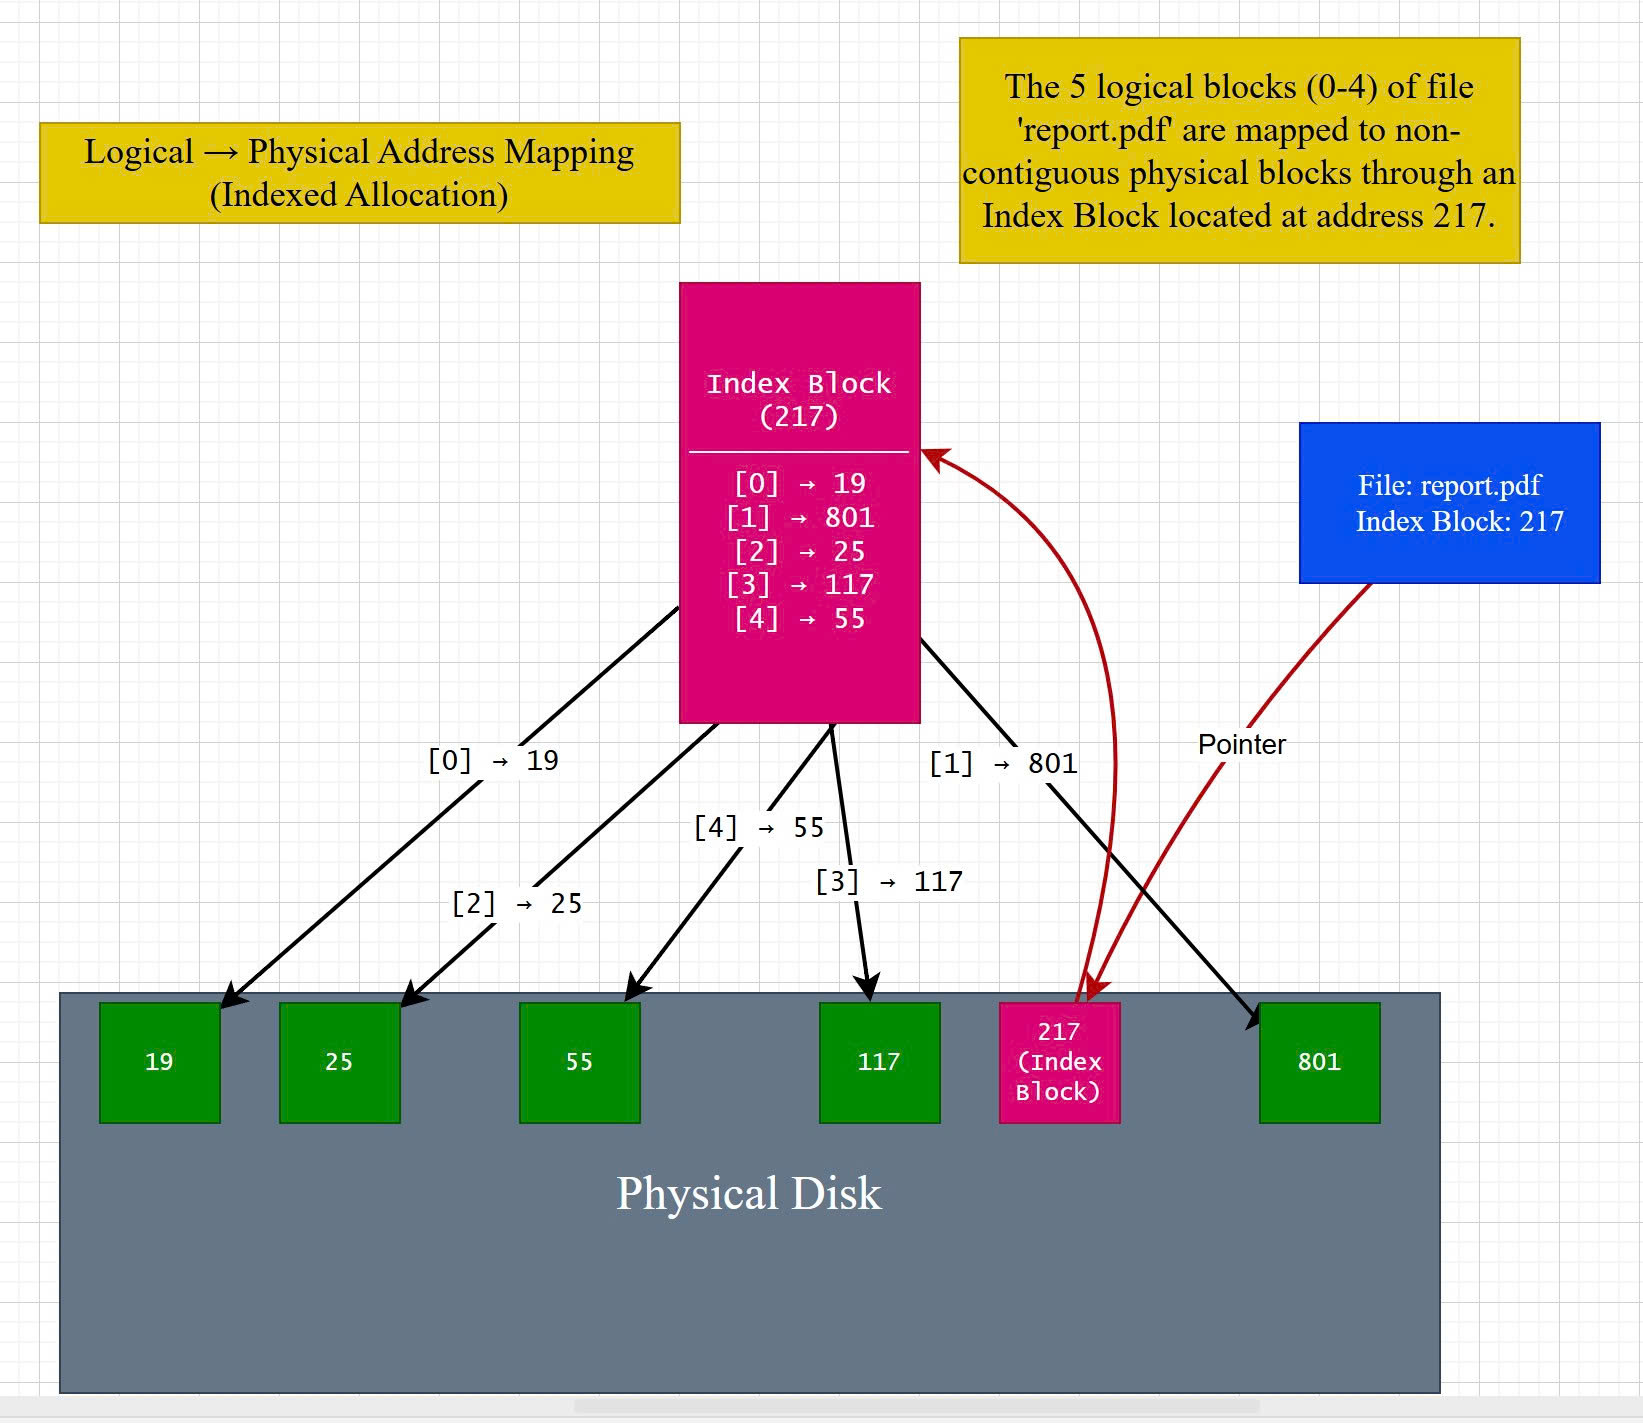
\includegraphics[width=\textwidth]{image/diagram mapping Indexed Allocation.jpg}
    \caption{Logical $\rightarrow$ Physical Address Mapping using Indexed Allocation.}
    \label{fig:indexed_allocation_diagram}
\end{figure}

\subsubsection{Hybrid Approaches and Modern Solutions}
Since all methods have limitations, recent researches have considered hybrid approaches combining the strengths of several methods. One such is the “Hybrid Indexed and Linked List File Allocation System” by Rahman and Siddiqua. This scheme introduces a novel flexible approach: for small size file (e.g., less than 10 blocks) it employs the linked allocation scheme which is to avoid space wastage for a useless index block. When a file exceeds a certain size, the system switches to indexed allocation to provide better random access for large files \parencite{IRJMETS2021}. Such a policy is representative of an attempt to improve allocation performance on the characteristics of each file rather than with one rule for the entire file system. 

%======================================================================
% PHẦN 2.4: LẬP LỊCH TRUY XUẤT ĐĨA
%======================================================================
% % https://calculator.pisqre.com/disk-scheduling
% % https://seektime.app/ : tính vẽ đường này nọ cũng đẹp
% % TODO: BẮT BUỘC THÊM PHẦN TÍNH TOÁN VÀ SƠ ĐỒ GANTT TẠI ĐÂY
% % Dựa trên dàn bài nâng cao, bạn cần thêm một ví dụ cụ thể:
% % - Example Request Queue: 98, 183, 37, 122, 14, 124, 65, 67
% % - Starting position: 53
% % - Tính toán Total Head Movement cho từng thuật toán.
% % - Vẽ sơ đồ Gantt minh họa cho mỗi thuật toán.
% 
\includegraphics[width=\textwidth]{placeholder.png}

\subsection{Disk I/O Scheduling}

One of the primary causes of a performance "bottleneck" for traditional computer systems is the difference in speed between the CPU/main memory and mechanical storage media such as hard disk drives (HDDs) \parencite{Pokharel2021}. For an HDD, data access time has two fundamental parts: seek time—the duration for the read/write head to move to the correct cylinder, and rotational latency—the duration for the sector requested to rotate to the location of the head. Of these, seek time will be the most costly and fluctuating part \parencite{KansalDiskScheduling}. Thus, in a system that supports multitasking where multiple processes concurrently initiate I/O requests, the operating system should have a facility to schedule the completion of the same. It is called disk scheduling, where its foremost aim is to minimize head movement and therefore reduce the average response time as well as increase the system throughput \parencite{GeeksForGeeks2025IO}. The following algorithms are the most widely used methods.

\subsubsection{FCFS (First-Come, First-Served)}
This is the simplest scheduling algorithm, in which I/O requests are serviced in the exact order they arrive. FCFS ensures absolute fairness because no request suffers from starvation. However, it does not perform any optimization regarding head movement. This can lead to very large and inefficient back-and-forth movements of the head across the disk surface, significantly degrading the overall performance of the system \parencite{GeeksForGeeks2025IO}.

\subsubsection{SSTF (Shortest Seek Time First)}
The SSTF algorithm selects the request with the shortest seek time (distance) from the current head position to service next. Essentially, it prioritizes the "closest" requests, regardless of when they arrived. SSTF significantly improves upon FCFS by minimizing the total distance the head travels. However, its major drawback is the potential for starvation: requests at distant cylinders (at the inner or outer edge of the disk) may wait indefinitely if new requests continuously arrive near the current head's position \parencite{GeeksForGeeks2025IO} \parencite{KansalDiskScheduling}.

\subsubsection{SCAN (Elevator Algorithm)}
The SCAN algorithm, also known as the elevator algorithm, works by having the head move from one end of the disk toward the other, servicing all requests in its path. Upon reaching the other end, it reverses direction and repeats the process. SCAN resolves the starvation problem of SSTF because it guarantees it will pass all cylinders. However, it has a slight bias towards the middle cylinders and can cause long waiting times for requests that the head has just passed \parencite{GeeksForGeeks2025IO}.

\subsubsection{C-SCAN (Circular SCAN)}
C-SCAN is an extension of SCAN that is implemented to provide a more balanced waiting time. Similar to SCAN, the head moves from one end of the disk to the other, servicing requests. But when it arrives at the other end, rather than reversing direction, it takes a gigantic "jump" and returns to the starting position and goes on scanning in the same direction. By fulfilling requests in one direction, C-SCAN ensures that requests at the outermost and innermost cylinders get more evenly spaced wait times, eliminating SCAN algorithm bias \parencite{KansalDiskScheduling, GeeksForGeeks2025IO}.

\subsubsection{Quantitative Analysis with an Example}
Assume there is a queue of requests to access the following cylinders: 98, 183, 37, 122, 14, 124, 65, 67. The disk has 200 cylinders (ranging between 0 and 199), and the beginning position of the head is cylinder 53.

\paragraph{FCFS:}
\begin{itemize}
    \item \textbf{Sequence:} 53 \(\rightarrow\) 98 \(\rightarrow\) 183 \(\rightarrow\) 37 \(\rightarrow\) 122 \(\rightarrow\) 14 \(\rightarrow\) 124 \(\rightarrow\) 65 \(\rightarrow\) 67
    \item \textbf{Total Head Movement:} (98-53) + (183-98) + (183-37) + (122-37) + (122-14) + (124-14) + (124-65) + (67-65) = \textbf{640} cylinders.
\end{itemize}

\paragraph{SSTF:}
\begin{itemize}
    \item \textbf{Sequence:} 53 \(\rightarrow\) 65 \(\rightarrow\) 67 \(\rightarrow\) 37 \(\rightarrow\) 14 \(\rightarrow\) 98 \(\rightarrow\) 122 \(\rightarrow\) 124 \(\rightarrow\) 183
    \item \textbf{Total Head Movement:} (65-53) + (67-65) + (67-37) + (37-14) + (98-14) + (122-98) + (124-122) + (183-124) = \textbf{236} cylinders.
\end{itemize}

\paragraph{SCAN (assuming moving towards 199 initially):}
\begin{itemize}
    \item \textbf{Sequence:} 53 \(\rightarrow\) 65 \(\rightarrow\) 67 \(\rightarrow\) 98 \(\rightarrow\) 122 \(\rightarrow\) 124 \(\rightarrow\) 183 \(\rightarrow\) 199 \(\rightarrow\) 37 \(\rightarrow\) 14
    \item \textbf{Total Head Movement:} (199 - 53) + (199 - 14) = 146 + 185 = \textbf{331} cylinders.
\end{itemize}

\paragraph{C-SCAN (assuming moving towards 199 initially):}
\begin{itemize}
    \item \textbf{Sequence:} 53 \(\rightarrow\) 65 \(\rightarrow\) 67 \(\rightarrow\) 98 \(\rightarrow\) 122 \(\rightarrow\) 124 \(\rightarrow\) 183 \(\rightarrow\) 199 \(\rightarrow\) 0 \(\rightarrow\) 14 \(\rightarrow\) 37
    \item \textbf{Total Head Movement:} (199 - 53) + (199 - 0) + (37 - 0) = 146 + 199 + 37 = \textbf{382} cylinders.
\end{itemize}

% TODO: BẮT BUỘC THÊM BIỂU ĐỒ GANTT TẠI ĐÂY
% Bạn có thể dùng công cụ draw.io để vẽ các biểu đồ minh họa chuyển động của đầu đọc cho từng thuật toán,
% sau đó chèn vào file LaTeX dưới dạng hình ảnh.


%======================================================================
% PHẦN 2.5: CÁC KỸ THUẬT TĂNG HIỆU NĂNG VÀ ĐỘ TIN CẬY (PHIÊN BẢN NÂNG CAO)
%======================================================================

\subsection{Performance \& Reliability Techniques}
In addition to optimizing the physical access order, the operating system also implements techniques at the logical layer to enhance performance and ensure data integrity. Three of the most important and popular mechanisms in modern file systems are caching, buffering, and journaling.

\subsubsection{Caching and Buffering}
Although often used interchangeably, buffering and caching are two distinct concepts with different objectives aimed at addressing the I/O performance bottleneck.

\textbf{Buffering} is a technique that uses a buffer (a block of memory) to store data temporarily as it is being transferred from one device operating at a different rate to another. Its primary purpose is to "smooth" data flow and allow processes to continue without having to wait for the physical I/O operation to complete. For example, when an application is performing a write operation, the data can be duplicated into the kernel buffer and the system call will return at once. The kernel will thereafter schedule to write the data out of the buffer to the disk in the background. The buffer data is the original data which is held pending for processing and would typically exist only for a short period of time \parencite{GeeksForGeeks2025BufferCache}.

On the other hand, \textbf{caching} is the act of \textit{duplicating} a heavily used portion of data from a slow storage device (like an HDD) to a quicker memory area (like RAM). Caching is a bid to reduce future \textit{read} access latency. When a read request is made, the system first checks the cache. If the data is in the cache (a cache hit), it is displayed immediately without needing to access the slow device. Otherwise (a cache miss), the data is loaded from the slow device, displayed for the request, and simultaneously a copy of it is stored in the cache to serve future accesses \parencite{GeeksForGeeks2025BufferCache}. Both these mechanisms are usually combined into a single memory management system by the majority of modern operating systems, usually called a \textbf{unified page cache}, to allocate dynamically memory among processes and I/O operations of the file system \parencite{Silberschatz2018}.

\subsubsection{Journaling}
One of the largest problems a file system has is to be in a stable state during an immediate failure, say a power failure or system crash. A simple logical operation such as file deletion can be many individual physical writes to metadata (e.g., marking a bitmap, updating an inode, updating directory entries).. If something goes wrong between these operations, the file system will be in an inconsistent state, and this inconsistency can lead to data loss or storage leaks of space \parencite{LibreTextsJournaling}. Recovery of an inconsistent file system by commands like fsck typically takes very much time because it needs to scan the entire metadata structure of the disk.

In order to solve this problem, modern file systems use a method called journaling, or write-ahead logging. The idea is simple: before writing the changes into the underlying file system structure, a description of the "intent" of the changes is written to a special area called the \textbf{journal}. It is only when this transaction has been safely recorded in the journal and marked as committed that the system initiates the \textbf{checkpointing} process—i.e., writing the actual changes to their permanent residence. On a crash, after rebooting, the system only needs to read the journal and "replay" those transactions that were committed but didn't complete checkpointing to bring the file system to a consistent state very quickly \parencite{Prabhakaran2005journaling, Jones2008Anatomy}.

Journaling file systems typically implement three different operating modes, which represent the trade-off between performance and the level of data protection:

\begin{itemize}
    \item \textbf{Writeback Mode:} Đây là chế độ có hiệu năng cao nhất nhưng rủi ro nhất. Trong chế độ này, chỉ có metadata được ghi vào journal. Dữ liệu của file được ghi trực tiếp vào vị trí cố định của nó mà không có bất kỳ sự đồng bộ nào với việc ghi metadata. Điều này có nghĩa là metadata có thể được ghi trước hoặc sau dữ liệu. Nếu xảy ra sự cố, hệ thống file có thể phục hồi về trạng thái metadata nhất quán, nhưng dữ liệu của file có thể bị cũ hoặc chứa dữ liệu rác \parencite{Jones2008Anatomy}.

    \item \textbf{Ordered Mode:} Đây là chế độ mặc định trên hầu hết các hệ thống Linux (bao gồm cả ext3 và ext4) và là một sự cân bằng tốt giữa hiệu năng và an toàn. Tương tự như writeback, chỉ có metadata được ghi vào journal. Tuy nhiên, chế độ này áp đặt một trật tự ghi nghiêm ngặt: dữ liệu của file \textit{phải} được ghi vào vị trí cố định của nó \textit{trước khi} metadata liên quan đến nó được commit vào journal. Trật tự này đảm bảo rằng metadata sẽ không bao giờ trỏ đến các khối dữ liệu chưa được ghi hoặc chứa dữ liệu rác, do đó ngăn ngừa được tình trạng hỏng dữ liệu sau khi phục hồi, mặc dù vẫn có thể mất các cập nhật mới nhất \parencite{Prabhakaran2005journaling}.

    \item \textbf{Data Mode (Full Data Journaling):} Đây là chế độ an toàn nhất nhưng cũng chậm nhất. Trong chế độ này, cả \textbf{metadata và dữ liệu} của file đều được ghi vào journal trước khi được checkpoint. Điều này có nghĩa là mỗi khối dữ liệu được ghi hai lần: một lần vào journal và một lần vào vị trí cuối cùng của nó. Chế độ này đảm bảo tính nhất quán ở mức cao nhất; sau sự cố, file sẽ ở trạng thái cũ hoặc mới một cách toàn vẹn. Tuy nhiên, việc ghi kép này làm giảm đáng kể thông lượng ghi của hệ thống \parencite{Jones2008Anatomy}.
\end{itemize}



%======================================================================
% PHẦN 3: CASE STUDY NTFS
%======================================================================

\section{Analysis \& Case Study: NTFS Deep Dive}

%======================================================================
% PHẦN 3.1: PHÂN TÍCH SO SÁNH TỔNG HỢP
%======================================================================

\subsection{Comparative Analysis}

Sau khi đã khảo sát các khái niệm lý thuyết và kiến trúc cơ bản của ba hệ thống file tiêu biểu trong Phần 2, phần này sẽ tiến hành tổng hợp và so sánh trực tiếp các đặc tính của chúng dựa trên các tiêu chí quan trọng về hiệu năng, độ tin cậy, bảo mật và các trường hợp sử dụng thực tế. Phân tích này sẽ làm nổi bật sự đánh đổi (trade-offs) giữa các thiết kế và tạo tiền đề cho phần nghiên cứu điển hình chuyên sâu về NTFS.

\subsubsection{Performance Comparison}
Hiệu năng của một hệ thống file phụ thuộc rất lớn vào cách nó quản lý việc cấp phát khối và metadata. Dựa trên kiến trúc, chúng ta có thể so sánh hiệu năng lý thuyết của FAT32, ext4 và NTFS trong các kịch bản sau:
\begin{itemize}
    \item \textbf{Truy cập tuần tự (Sequential Access):} Cả ext4 và NTFS đều cho hiệu năng vượt trội trong kịch bản này. ext4 sử dụng cơ chế \textbf{extents}, cho phép nó cấp phát các dải khối lớn và liền kề, giảm thiểu đáng kể chuyển động của đầu đọc \parencite{Dhjaku2019}. NTFS cũng có các thuật toán cấp phát thông minh để giữ cho các file lớn càng liền kề càng tốt. Ngược lại, FAT32, với bản chất danh sách liên kết, rất dễ bị phân mảnh, khiến cho việc đọc một file lớn, tuần tự có thể yêu cầu nhiều thao tác tìm kiếm (seek) tốn kém.

    \item \textbf{Truy cập ngẫu nhiên (Random Access):} Các hệ thống file dựa trên chỉ mục như ext4 và NTFS lại chiếm ưu thế. Cấu trúc inode với các con trỏ đa cấp của ext4 và kiến trúc MFT tập trung của NTFS cho phép hệ thống nhanh chóng định vị bất kỳ khối dữ liệu nào của file chỉ qua một vài lần truy cập metadata. FAT32, một lần nữa, tỏ ra yếu thế vì việc truy cập một khối ở giữa file đòi hỏi phải duyệt qua chuỗi con trỏ từ đầu \parencite{Silberschatz2018}.

    \item \textbf{Xử lý file nhỏ:} NTFS có một lợi thế đặc biệt với các file rất nhỏ nhờ tính năng \textbf{dữ liệu nội trú (resident data)}. Nếu dữ liệu của một file đủ nhỏ, nó có thể được lưu trữ trực tiếp bên trong bản ghi MFT của file đó, loại bỏ hoàn toàn nhu cầu truy cập vào các khối dữ liệu bên ngoài và mang lại tốc độ truy cập cực nhanh \parencite{Tanenbaum2014}. ext4 cũng xử lý file nhỏ hiệu quả bằng cách cố gắng gom chúng vào cùng một block group để tăng tính cục bộ (locality).

    \item \textbf{Xử lý file lớn:} Giới hạn kích thước file 4GB của FAT32 khiến nó không còn phù hợp. Cả ext4 và NTFS đều hỗ trợ kích thước file và phân vùng cực lớn, lên đến hàng Terabyte và Exabyte, đáp ứng tốt các nhu-cầu lưu trữ hiện đại \parencite{Dhjaku2019}.
\end{itemize}

\subsubsection{Security and Reliability}
Về độ tin cậy và bảo mật, sự khác biệt giữa các hệ thống file là rất rõ rệt.
\begin{itemize}
    \item \textbf{Độ tin cậy (Reliability):} Lợi thế lớn nhất của ext4 và NTFS so với FAT32 là việc hỗ trợ \textbf{journaling}. Như đã phân tích ở Mục 2.5.3, cơ chế ghi nhật ký đảm bảo rằng hệ thống file có thể nhanh chóng phục hồi về một trạng thái nhất quán sau sự cố đột ngột, giảm thiểu nguy cơ hỏng cấu trúc metadata và rút ngắn đáng kể thời gian kiểm tra đĩa (fsck) khi khởi động lại \parencite{Prabhakaran2005journaling}. FAT32 không có cơ chế này, khiến nó dễ bị lỗi và mất dữ liệu hơn.

    \item \textbf{Bảo mật (Security):} FAT32 chỉ cung cấp các cơ chế bảo mật rất cơ bản ở cấp độ chia sẻ (share-level). Ngược lại, ext4 và NTFS đều được xây dựng cho các hệ điều hành đa người dùng. ext4 sử dụng mô hình phân quyền \textbf{POSIX} kinh điển của UNIX, định nghĩa quyền truy cập cho ba lớp: người sở hữu (owner), nhóm sở hữu (group), và những người khác (other). Trong khi đó, NTFS triển khai một mô hình linh hoạt và mạnh mẽ hơn nhiều gọi là \textbf{Access Control Lists (ACLs)}. Với ACLs, quản trị viên có thể gán hoặc từ chối các quyền cụ thể (đọc, ghi, thực thi, xóa, v.v.) cho nhiều người dùng và nhóm khác nhau trên cùng một file hoặc thư mục, cho phép kiểm soát truy cập ở mức độ chi tiết hơn hẳn \parencite{Bundele2018}.
\end{itemize}

\subsubsection{Use Case Scenarios}
Từ những phân tích trên, vai trò của mỗi hệ thống file trong các môi trường khác nhau được định hình rõ ràng:
\begin{itemize}
    \item \textbf{FAT32:} Mặc dù đã lỗi thời về mặt công nghệ, sự đơn giản và khả năng tương thích gần như toàn cầu giúp FAT32 (và người kế nhiệm là exFAT) vẫn là lựa chọn số một cho các thiết bị lưu trữ di động cần trao đổi dữ liệu giữa nhiều nền tảng khác nhau, như USB flash drives và thẻ nhớ SD.

    \item \textbf{ext4:} Là hệ thống file bản địa của hệ sinh thái Linux, ext4 là sự lựa chọn mặc định cho hầu hết mọi thứ, từ máy chủ doanh nghiệp, máy tính để bàn cho đến các thiết bị nhúng chạy Linux. Nó cung cấp một sự cân bằng tuyệt vời giữa hiệu năng, độ tin cậy và sự ổn định trong một môi trường mã nguồn mở.

    \item \textbf{NTFS:} Là nền tảng không thể thiếu của hệ điều hành Windows. Với bộ tính năng doanh nghiệp phong phú, bao gồm bảo mật ACLs, mã hóa, nén dữ liệu và khả năng phục hồi mạnh mẽ, NTFS là lựa chọn mặc định cho các ổ đĩa hệ thống và dữ liệu trong môi trường Windows, đặc biệt là các máy trạm và máy chủ đòi hỏi độ tin cậy và khả năng quản trị cao.
\end{itemize}

Với việc đã thiết lập một cơ sở so sánh tổng quan, báo cáo sẽ tiếp tục đi sâu vào nghiên cứu điển hình về kiến trúc NTFS để minh họa chi tiết hơn các khái niệm đã được thảo luận.


%======================================================================
% PHẦN 3.2: CASE STUDY: PHÂN TÍCH CHUYÊN SÂU VỀ NTFS (ĐÃ SỬA LỖI)
%======================================================================

\subsection{Case Study: A Deep Dive into the New Technology File System (NTFS)}

\subsubsection{Introduction}
Được giới thiệu lần đầu tiên cùng Windows NT 3.1, \textbf{New Technology File System (NTFS)} được Microsoft thiết kế từ đầu để thay thế hệ thống file FAT đã lỗi thời. Mục tiêu của NTFS là cung cấp một nền tảng lưu trữ mạnh mẽ, đáp ứng các yêu cầu ngày càng cao của môi trường doanh nghiệp về hiệu năng, độ tin cậy, bảo mật và khả năng quản lý các ổ đĩa dung lượng lớn \parencite{Shafiei2012}. Kể từ đó, NTFS đã trở thành hệ thống file mặc định và không thể thiếu trên tất cả các phiên bản hệ điều hành Windows hiện đại.

\subsubsection{Core Architecture: The Master File Table (MFT)}
Kiến trúc của NTFS xoay quanh một triết lý thiết kế trung tâm: \textit{"mọi thứ trên volume đều là một file"} \parencite{Shafiei2012}. Điều này bao gồm cả chính các cấu trúc metadata của hệ thống file. Trái tim của kiến trúc này là một file đặc biệt có tên là \textbf{\$MFT}, hay \textbf{Master File Table}. Về bản chất, MFT là một cơ sở dữ liệu quan hệ, chứa ít nhất một bản ghi (record) --- thường có kích thước cố định là 1024 byte --- cho mỗi file và thư mục tồn tại trên volume \parencite{HarvardCS161Journaling}.

Mỗi bản ghi MFT chứa một tập hợp các \textbf{thuộc tính (attributes)} mô tả đầy đủ về file hoặc thư mục đó. Các thuộc tính này bao gồm metadata cơ bản như \texttt{\$STANDARD\_INFORMATION} (chứa dấu thời gian, quyền sở hữu) và \texttt{\$FILE\_NAME} (tên file), cũng như một thuộc tính đặc biệt quan trọng là \texttt{\$DATA} \parencite{Shafiei2012}. Một trong những tối ưu hóa hiệu năng độc đáo nhất của NTFS nằm ở cách nó xử lý thuộc tính \texttt{\$DATA}:
\begin{itemize}
    \item \textbf{Resident Data (Dữ liệu nội trú):} Đối với các file có kích thước rất nhỏ, thay vì cấp phát một khối riêng trên đĩa, toàn bộ dữ liệu của file sẽ được lưu trữ trực tiếp bên trong thuộc tính \texttt{\$DATA} ngay trong bản ghi MFT. Việc này loại bỏ hoàn toàn một thao tác truy cập đĩa, giúp đọc các file nhỏ với tốc độ cực nhanh \parencite{CIRCL2023}.
    
    \item \textbf{Non-resident Data (Dữ liệu không nội trú):} Khi dữ liệu của file vượt quá không gian còn lại trong bản ghi MFT, nó sẽ được chuyển thành dạng không nội trú. Lúc này, thuộc tính \texttt{\$DATA} không còn chứa dữ liệu nữa mà thay vào đó chứa các con trỏ trỏ đến các "dải" (extents) của các cluster trên đĩa nơi dữ liệu thực sự được lưu trữ \parencite{HarvardCS161Journaling}.
\end{itemize}

\subsubsection{Analysis of Advanced Features}
Ngoài kiến trúc MFT, sức mạnh của NTFS còn đến từ bộ tính năng doanh nghiệp phong phú được tích hợp sẵn.

\paragraph{A. Journaling and Recovery (\texttt{\$LogFile}):}
NTFS là một hệ thống file journaling hoàn chỉnh, đảm bảo tính nhất quán của volume ngay cả khi xảy ra sự cố đột ngột. Cơ chế này được triển khai thông qua một file metadata đặc biệt có tên là \textbf{\texttt{\$LogFile}} \parencite{Shafiei2012}. Không giống như ext3 sử dụng "physical logging" (ghi lại toàn bộ khối metadata bị thay đổi), NTFS triển khai một hình thức ghi nhật ký tinh vi hơn gọi là \textbf{operation logging} (hay redo/undo logging). Trong mô hình này, journal không ghi lại toàn bộ khối dữ liệu mà chỉ ghi lại các thao tác logic mô tả sự thay đổi ("redo" - làm lại) và cách để hoàn tác thay đổi đó ("undo" - làm lại) \parencite{HarvardCS161Journaling}. Khi một giao dịch được cam kết, hệ điều hành sẽ thực hiện các thay đổi. Nếu hệ thống gặp sự cố, trong quá trình phục hồi, NTFS sẽ quét \texttt{\$LogFile}, "redo" lại các giao dịch đã hoàn thành và "undo" các giao dịch chưa hoàn thành, đảm bảo metadata của hệ thống file nhanh chóng trở lại trạng thái nhất quán.

\paragraph{B. Security: Access Control Lists (ACLs):}
NTFS cung cấp một mô hình bảo mật cực kỳ linh hoạt và chi tiết thông qua \textbf{Access Control Lists (ACLs)}. Mỗi file và thư mục trên một volume NTFS đều có một ACL, là một danh sách chứa các \textbf{Access Control Entries (ACEs)}. Mỗi ACE xác định một người dùng hoặc một nhóm cụ thể và định nghĩa một tập hợp các quyền (permissions) --- chẳng hạn như Đọc, Ghi, Thực thi --- được \textit{Cho phép (Allow)} hoặc \textit{Từ chối (Deny)} \parencite{SettingAccessControlLists}. Mô hình này, được gọi là Discretionary Access Control (DAC), cho phép quản trị viên kiểm soát truy cập ở mức độ rất chi tiết, vượt xa mô hình ba lớp (owner, group, other) của POSIX/Linux. Một quy tắc quan trọng trong NTFS là một ACE "Deny" sẽ luôn được ưu tiên hơn một ACE "Allow", cung cấp một cơ chế mạnh mẽ để khóa quyền truy cập một cách tường minh \parencite{Allison1998}.

\paragraph{C. Other Enterprise Features:}
\begin{itemize}
    \item \textbf{Volume Shadow Copy Service (VSS):} Là một framework mạnh mẽ cho phép tạo các "ảnh chụp" (snapshot) nhất quán tại một thời điểm của một volume, ngay cả khi các file trên đó đang được sử dụng. VSS điều phối giữa các ứng dụng, hệ thống file và nhà cung cấp phần cứng để tạm thời đóng băng các hoạt động ghi, tạo snapshot, sau đó cho phép hoạt động trở lại. Cơ chế này (thường sử dụng kỹ thuật copy-on-write) là nền tảng cho các tính năng như sao lưu trực tuyến (online backup) và System Restore trong Windows \parencite{MicrosoftVSS}.
    \item \textbf{Encryption and Compression:} NTFS hỗ trợ mã hóa và nén dữ liệu ở cấp độ file system một cách minh bạch với người dùng. \textbf{Encrypting File System (EFS)} cho phép người dùng mã hóa các file/thư mục bằng cơ chế mã hóa khóa công khai, đảm bảo chỉ người dùng đó mới có thể giải mã dữ liệu \parencite{WafaTech2025EFS}. Tính năng nén, mặt khác, giúp tiết kiệm không gian đĩa bằng cách nén dữ liệu một cách tự động khi ghi và giải nén khi đọc.
\end{itemize}

\subsubsection{Evaluation and Limitations}
\textbf{Điểm mạnh:} Kiến trúc NTFS thể hiện rõ sự vượt trội về độ tin cậy thông qua journaling, bảo mật mạnh mẽ với ACLs, và hiệu năng linh hoạt, xử lý tốt cả file nhỏ (với resident data) và file rất lớn. Bộ tính năng doanh nghiệp phong phú như VSS và EFS làm cho nó trở thành một nền tảng vững chắc cho các môi trường đòi hỏi cao.

\textbf{Điểm yếu:} Sự phức tạp của MFT và các tính năng nâng cao đi kèm với một lượng overhead metadata đáng kể so với các hệ thống file đơn giản hơn. Tuy nhiên, hạn chế lớn nhất của NTFS trong môi trường đa nền tảng là khả năng tương thích. Mặc dù các hệ điều hành như Linux và macOS có thể đọc được phân vùng NTFS, khả năng ghi dữ liệu một cách ổn định và hiệu quả thường phụ thuộc vào các driver của bên thứ ba (ví dụ: NTFS-3G), vốn được phát triển thông qua kỹ thuật dịch ngược và có thể không đạt được hiệu năng như driver gốc trên Windows \parencite{Dhjaku2019}.


%======================================================================
% PHẦN 4: BÀN LUẬN (DISCUSSION)
%======================================================================

\section{Discussion}
Các phân tích lý thuyết và nghiên cứu điển hình đã cho thấy một bức tranh đa chiều về lĩnh vực quản lý hệ thống file và lưu trữ. Rõ ràng, không có một giải pháp "tốt nhất" cho mọi trường hợp; thay vào đó, sự lựa chọn tối ưu luôn là một sự cân nhắc kỹ lưỡng giữa các yếu tố đánh đổi (trade-offs) về hiệu năng, độ tin cậy, chi phí và tính tương thích.

\subsection{Key Findings Interpretation and Design Trade-offs}
Kết quả phân tích cho thấy các hệ thống file truyền thống đã phát triển các cơ chế phức tạp để đảm bảo tính nhất quán và hiệu năng. \textbf{Journaling} là một ví dụ điển hình: nó là một "game-changer" cho độ tin cậy, nhưng cơ chế này về bản chất làm tăng gấp đôi lượng ghi cho các hoạt động siêu dữ liệu (metadata) và đôi khi cả dữ liệu người dùng \parencite{Lu2013Extending}. Sự đánh đổi này, vốn đã được chấp nhận trên HDD, lại trở thành một vấn đề nghiêm trọng hơn trên các thiết bị lưu trữ hiện đại. Tương tự, các phương pháp cấp phát là một sự cân bằng giữa hiệu năng truy cập và hiệu quả sử dụng không gian, nơi cấp phát theo chỉ mục (indexed allocation) được ưa chuộng vì tính linh hoạt của nó.

\subsection{The Impact of Modern Storage: SSDs and New Challenges}
Sự trỗi dậy của các thiết bị lưu trữ thể rắn (SSDs) đã định hình lại hoàn toàn các giả định nền tảng của việc quản lý lưu trữ. Đặc điểm vật lý của bộ nhớ flash NAND, đặc biệt là việc không có các bộ phận cơ khí chuyển động, đã làm cho các thuật toán lập lịch đĩa kinh điển (SCAN, C-SCAN, LOOK) trở nên lỗi thời, vì thời gian truy cập đến bất kỳ khối logic nào gần như là không đổi.

Tuy nhiên, kiến trúc của SSD lại giới thiệu những thách thức mới và phức tạp hơn mà các hệ thống file phải đối mặt. Khác với HDD, dữ liệu trên SSD không thể được ghi đè trực tiếp. Thay vào đó, các đơn vị bộ nhớ (page) phải được xóa trước khi ghi lại, và thao tác xóa chỉ có thể thực hiện trên các đơn vị lớn hơn nhiều gọi là "block" \parencite{Viking2017AN0035, Lu2013Extending}. Ràng buộc này là nguồn gốc của hai vấn đề lớn:

\begin{itemize}
    \item \textbf{Write Amplification (Khuếch đại ghi - WA):} Đây là hiện tượng lượng dữ liệu được ghi vật lý xuống chip flash lớn hơn lượng dữ liệu mà hệ điều hành yêu cầu ghi. Nguyên nhân chính là do quá trình \textbf{dọn rác (garbage collection - GC)}, trong đó bộ điều khiển SSD phải đọc các page hợp lệ từ một block, sao chép chúng sang một block mới, sau đó mới xóa block cũ để chuẩn bị cho các lần ghi trong tương lai. Kết quả là, một thao tác ghi logic nhỏ có thể gây ra nhiều thao tác đọc và ghi vật lý, làm giảm đáng kể hiệu năng và quan trọng hơn là tuổi thọ của ổ đĩa (được đo bằng DWPD hoặc TBW) \parencite{Viking2017AN0035}. Các yếu tố như ghi ngẫu nhiên, không gian trống thấp, và việc thiếu lệnh TRIM đều làm tăng đáng kể hệ số WA.
    \item \textbf{Wear Leveling (Cân bằng độ mòn):} Mỗi ô nhớ flash có một số chu kỳ ghi/xóa (P/E cycles) hữu hạn. Để tối đa hóa tuổi thọ, bộ điều khiển SSD phải triển khai các thuật toán cân bằng độ mòn để phân bổ các thao tác ghi đều trên toàn bộ các block nhớ.
\end{itemize}

Các hệ thống file truyền thống, với các cơ chế như journaling và cập nhật metadata thường xuyên, có thể vô tình làm trầm trọng thêm vấn đề khuếch đại ghi \parencite{Lu2013Extending}. Hơn nữa, một thách thức tinh vi khác nằm ở lệnh \textbf{FLUSH}, vốn được sử dụng để đảm bảo dữ liệu được ghi bền vững từ bộ đệm (buffer) của thiết bị xuống phương tiện lưu trữ. Trên các SSD hiện đại với bộ đệm DRAM lớn, một lệnh FLUSH "lump-sum" (ghi toàn bộ) có thể buộc hàng gigabyte dữ liệu không liên quan phải được ghi xuống, làm chậm đáng kể các hoạt động quan trọng và gây ra độ trễ lớn (long tail latency), đặc biệt trong các môi trường đa nhiệm \parencite{Yeon2018RFLUSH}. Điều này cho thấy sự tương tác giữa phần mềm (hệ điều hành/hệ thống file) và phần cứng (bộ điều khiển SSD) ngày càng trở nên quan trọng và đòi hỏi những cách tiếp cận mới để tối ưu hóa hiệu năng.

%======================================================================
% PHẦN 5: KẾT LUẬN (CONCLUSION)
%======================================================================

\section{Conclusion}
Báo cáo này đã thực hiện một cuộc khảo sát toàn diện về các nguyên tắc cơ bản và các kỹ thuật nâng cao trong lĩnh vực quản lý hệ thống file và lưu trữ của hệ điều hành. Qua việc phân tích lý thuyết, so sánh các kiến trúc, và thực hiện một nghiên cứu điển hình, các mục tiêu đề ra ban đầu đã được hoàn thành một cách có hệ thống.

\subsection{Summary of Findings}
Báo cáo đã đáp ứng đầy đủ sáu yêu cầu cốt lõi của đề tài, từ việc \textbf{định nghĩa} các khái niệm nền tảng, \textbf{giải thích} và \textbf{so sánh} các kiến trúc hệ thống file và phương pháp cấp phát, \textbf{phân tích} các thuật toán lập lịch I/O, \textbf{mô tả} các kỹ thuật tối ưu hóa, cho đến việc tiến hành một \textbf{nghiên cứu điển hình} chuyên sâu về NTFS. Các sản phẩm được yêu cầu là Sơ đồ ánh xạ logic-vật lý và Bảng so sánh các hệ thống file cũng đã được tích hợp và trình bày trong báo cáo.

\subsection{Broader Implications and Future Outlook}
Phân tích đã chỉ ra rằng lĩnh vực quản lý lưu trữ đang trong một giai đoạn chuyển đổi sâu sắc, được thúc đẩy bởi sự thay đổi trong công nghệ phần cứng. Các hệ thống file không còn có thể hoạt động như một lớp trừu tượng hoàn toàn độc lập với thiết bị bên dưới. Thay vào đó, một tương lai hợp tác chặt chẽ hơn giữa hệ điều hành và bộ điều khiển lưu trữ là tất yếu.

Các hệ thống file thế hệ mới đang dẫn đầu xu hướng này bằng cách tích hợp các tính năng được thiết kế đặc biệt để giải quyết các thách thức về quy mô và tính toàn vẹn dữ liệu trên các phương tiện lưu trữ hiện đại.
\begin{itemize}
    \item \textbf{ZFS và Btrfs} đã trở nên phổ biến nhờ vào các tính năng đột phá. Cả hai đều sử dụng cơ chế \textbf{copy-on-write (CoW)}, giúp tạo snapshot và clone một cách cực kỳ hiệu quả. Quan trọng hơn, chúng tích hợp \textbf{checksum} cho cả dữ liệu và metadata ở mọi cấp độ, cho phép tự động phát hiện và sửa chữa các lỗi dữ liệu thầm lặng (silent data corruption) khi được sử dụng cùng với các cấu hình dự phòng (như mirroring hoặc RAID-Z). Chúng cũng hợp nhất việc quản lý volume và hệ thống file, mang lại sự linh hoạt cao hơn \parencite{Nfina2025BtrfsZFS}.
    \item \textbf{ReFS (Resilient File System)} của Microsoft cũng theo đuổi một triết lý tương tự, được định vị là người kế nhiệm của NTFS trong các môi trường máy chủ đòi hỏi tính toàn vẹn và khả năng phục hồi cao. ReFS sử dụng "luồng toàn vẹn" (integrity streams) để xác thực và tự động sửa chữa dữ liệu khi được kết hợp với Storage Spaces. Các tính năng như nhân bản khối (block cloning) và VDL thưa (sparse VDL) giúp tăng tốc đáng kể các hoạt động trên máy ảo, cho thấy sự tập trung rõ rệt vào các workload hiện đại \parencite{Microsoft2025ReFS}.
\end{itemize}
Những hệ thống này báo hiệu một tương lai nơi việc quản lý lưu trữ không chỉ nhanh hơn, mà còn thông minh hơn, linh hoạt hơn, và trên hết là đáng tin cậy hơn, có khả năng tự bảo vệ dữ liệu trước các lỗi phần cứng và phần mềm không thể tránh khỏi.





% Nội dung của phần Phân tích và Nghiên cứu điển hình...

%     \subsection{Comparative Analysis}
%     Tổng hợp so sánh từ Phần 2...

%     \subsection{Case Study: NTFS Architecture}
%     Phân tích sâu về NTFS, MFT, LogFile...

% \section{Discussion}
% Nội dung của phần Bàn luận...

%     \subsection{Key Findings Interpretation}
%     Diễn giải các kết quả chính...
    
%     \subsection{Design Trade-offs}
%     Phân tích các sự đánh đổi...
    
%     \subsection{Impact of Modern Storage (SSD/NVMe)}
%     Bàn luận về tác động của SSD...

% \section{Conclusion}
% Nội dung của phần Kết luận...

% --- PHẦN TÀI LIỆU THAM KHẢO ---
\newpage
\printbibliography[title={References}]

% % --- PHẦN TUYÊN BỐ SỬ DỤNG AI ---
% \newpage
% \section*{AI Usage Statement}
% % Viết tuyên bố sử dụng AI của nhóm bạn tại đây.
% Our team used AI tools (ChatGPT, Claude) for the following purposes: (1) Grammar and spelling checking, and (2) Explaining complex technical concepts during the research phase. All core content, analysis, diagrams, and conclusions were developed independently by team members through studying primary sources including OS textbooks, technical documentation, and academic papers. No AI-generated text was directly copied into the report.

\end{document}